\documentclass{article}
\usepackage{soul}
\usepackage{tikz}
\usepackage{xparse}

\def\primaer#1{\ul{#1}}
\def\fremd#1{{\setul{-0.9em}{}\ul{#1}}}
\NewDocumentEnvironment { rmodell }
{ +b }
{{\noindent\footnotesize\ttfamily#1}} {}

\usepackage[normalem]{ulem}  % for the dashed underline

% for text un key attributes
\newcommand{\key}[1]{\underline{#1}}

% for text in discriminator attributes
\def\discriminator{\bgroup
  \ifdim\ULdepth=\maxdimen  % Set depth based on font, if not set already
  \settodepth\ULdepth{(j}\advance\ULdepth.4pt\fi
  \markoverwith{\kern.15em
  \vtop{\kern\ULdepth \hrule width .3em}%
  \kern.15em}\ULon}

\usetikzlibrary{shapes.geometric}
\usetikzlibrary{positioning}

\tikzstyle{every entity} = []
\tikzstyle{every weak entity} = []
\tikzstyle{every attribute} = []
\tikzstyle{every relationship} = []
\tikzstyle{every link} = []
\tikzstyle{every isa} = []

\tikzstyle{er2} = [
  node distance = 2.3cm
]

\tikzstyle{weak} = [
  double,
  double distance=1pt,
]

\tikzstyle{entity} = [
  rectangle,
  draw,
  black,
  minimum width=6em,
  minimum height=3em,
  align=center,
  every entity,
]
\tikzstyle{weak entity} = [
  entity,
  double,
  double distance=1pt,
  every weak entity,
]

\tikzstyle{attribute} = [
  ellipse,
  draw,
  black,
  minimum width=5em,
  minimum height=2em,
  align=center,
  every attribute,
]

\tikzstyle{key attribute} = [
  attribute,
  font=\bfseries
  %node contents={\key{#1}},
]

\tikzstyle{discriminator} = [
  attribute,
  font=\itshape
]

\tikzstyle{relationship} = [
  diamond,
  draw,
  black,
  minimum width=2em,
  minimum width=4em,
  aspect=2,
  align=center,
  every relationship,
]

% identifying relationship
\tikzstyle{ident relationship} = [
  relationship,
  double,
  double distance=1pt,
]

\tikzstyle{isa} = [
  isosceles triangle,
  isosceles triangle apex angle=60,
  shape border rotate=90,
  draw,
  black,
  minimum size=3em,
  every isa,
]

\begin{document}

%-----------------------------------------------------------------------
%
%-----------------------------------------------------------------------

\section{Forstverwaltung}

66116 Datenbanksysteme / Softwaretechnologie (vertieft) 2016 Frühjahr.
Thema Nr. 1 / Teilaufgabe 1 / 1. Modellierung / Seite 2

\bigskip

\noindent
Für die bayerische Forstverwaltung wird eine Datenbank zur Erschließung
einer Jagd-Statistik benötigt. Gehen Sie dabei von folgendem Szenario
aus:

\begin{itemize}
\item Die Administration von Jagdgebieten obliegt den
Landkreisen. Jeder \emph{Landkreis} besitzt, neben seinem
\emph{Namen} (LName) und der \emph{Einwohnerzahl}, ein
eindeutiges \emph{KFZ-Kennzeichen} \texttt{(KFZKennzeichen)}.

\item Die Jagd findet in Jagdgebieten statt. Ein \emph{Jagdgebiet}
soll dem Landkreis \emph{zugeteilt} werden, indem es liegt.
Gehen Sie davon aus, dass Jagdgebiete nicht in mehreren Landkreisen
liegen können. Zusätzlich ist für jedes Jagdgebiet der
\emph{Name} \texttt{(JName)} und die \emph{Gesamtfläche}
zu speichern. Dabei ist zu beachten, dass die Namen nur innerhalb eines
einzelnen Landkreises eindeutig sind.

\item Die Erlaubnis zum Jagen wird durch einen \emph{Jagdschein}
erteilt. Dieser kann nur von einem Landkreis
\emph{ausgestellt} werden und \emph{beschränkt} sich
auf ein oder mehrere Jagdgebiete. Er wird durch eine
\emph{Jagdschein-Nummer} \texttt{(JSNR)} identifiziert und ist in
einem bestimmtem Zeitintervall gültig. Dieses soll über zwei Zeitpunkte
festgelegt werden (\emph{gültig von} \texttt{(gültigVon)},
\emph{gültig bis} \texttt{(gültigBis)}).

\item Ein \emph{Jäger} \emph{besitzt} genau einen
Jagdschein. Zu einem Jäger sollen \emph{Name},
\emph{Stadt}, \emph{Straße} und \emph{Hausnummer},
gespeichert werden. Da die Jagdtradition innerhalb einer Familie häufig
von einer zur nächsten Generation weitergegeben wird, kann es vorkommen,
dass Name und Adresse von zwei unterschiedlichen Jägern gleich ist
(z.\,B. Vater und Sohn). Aus diesem Grund ist eine eindeutige
\emph{Identifikationsnummer} \texttt{(JNR)} notwendig.

\item Um Statistiken erheben zu können, muss berücksichtigt werden,
welches \emph{Wild} von welchen Jägern zu welchem Zeitpunkt in
welchem Jagdgebiet \emph{erlegt} worden ist. Gehen Sie davon
aus, dass es mehrere Jäger geben kann, die gemeinsam ein Wild erlegen
(z.\,B. in einer Jagdgesellschaft). Zu einem Wild gehört die
\emph{Art} (z.\,B. Reh), die \emph{Größe}, das
\emph{Gewicht}, sowie eine eindeutige
\emph{Identifikationsnummer} \texttt{(WNR)}. Zusätzlich
unterscheidet man zwischen \emph{Haarwild} und \emph{Federwild},
wobei beim Haarwild der \emph{Typ des Gehörns}
\texttt{(GehörnTyp)} (z.\,B. Hirschgeweih) und beim Federwild die
\emph{Flügelspannweite} betrachtet werden soll.
\end{itemize}

\newpage

\begin{enumerate}

%%
% a)
%%

\item Entwerfen Sie für das beschriebene Szenario ein ER-Modell in
Chen-Notation. Bestimmen Sie hierzu:

\begin{itemize}
\item die Entity-Typen, die Relationship-Typen und jeweils deren
Attribute,

\item die Primärschlüssel der Entity-Typen, welche Sie anschließend in
das ER-Diagramm eintragen, und

\item die Funktionalitäten der Relationship-Typen.
\end{itemize}

\begin{center}
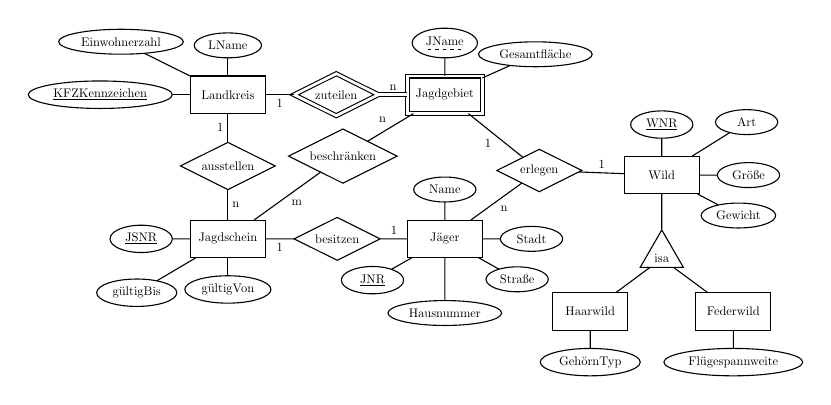
\begin{tikzpicture}[er2,scale=0.45,transform shape]
% Landkreis
\node[entity] (Landkreis) {Landkreis};
\node[attribute,above=0.5cm of Landkreis] {LName} edge (Landkreis);
\node[attribute,above left=1cm of Landkreis] {Einwohnerzahl} edge (Landkreis);
\node[attribute,left=0.5cm of Landkreis] {\key{KFZKennzeichen}} edge (Landkreis);

% Jagdgebiet
\node[weak entity,right=4cm of Landkreis] (Jagdgebiet) {Jagdgebiet};
\node[attribute,above=0.5cm of Jagdgebiet] {\discriminator{JName}} edge (Jagdgebiet);
\node[attribute,above right=0.5cm of Jagdgebiet] {Gesamtfläche} edge (Jagdgebiet);

% zuteilen
\node[ident relationship,right=0.8cm of Landkreis] {zuteilen}
  edge node[auto]{1} (Landkreis)
  edge[weak] node[auto]{n} (Jagdgebiet);

% Jagdschein
\node[entity,below=3cm of Landkreis] (Jagdschein) {Jagdschein};
\node[attribute,below=0.5cm of Jagdschein] {gültigVon} edge (Jagdschein);
\node[attribute,below left=1cm of Jagdschein] {gültigBis} edge (Jagdschein);
\node[attribute,left=0.5cm of Jagdschein] {\key{JSNR}} edge (Jagdschein);

% ausstellen
\node[relationship,below=0.8cm of Landkreis] {ausstellen}
  edge node[auto]{1} (Landkreis)
  edge node[auto]{n} (Jagdschein);

% Jäger
\node[entity,below=3cm of Jagdgebiet] (Jäger) {Jäger};
\node[attribute,above=0.5cm of Jäger] {Name} edge (Jäger);
\node[attribute,right=0.5cm of Jäger] {Stadt} edge (Jäger);
\node[attribute,below right=0.5cm of Jäger] {Straße} edge (Jäger);
\node[attribute,below=1.2cm of Jäger] {Hausnummer} edge (Jäger);
\node[attribute,below left=0.5cm of Jäger] {\key{JNR}} edge (Jäger);

% besitzen
\node[relationship,right=0.8cm of Jagdschein] {besitzen}
  edge node[auto]{1} (Jagdschein)
  edge node[auto]{1} (Jäger);

% Wild
\node[entity,below right=1.2cm and 4cm of Jagdgebiet] (Wild) {Wild};
\node[attribute,above right=1cm of Wild] {Art} edge (Wild);
\node[attribute,right=0.5cm of Wild] {Größe} edge (Wild);
\node[attribute,below right=0.5cm of Wild] {Gewicht} edge (Wild);
\node[attribute,above=0.5cm of Wild] {\key{WNR}} edge (Wild);

\node[relationship,above right=2cm of Jagdschein] {beschränken}
  edge node[auto]{m} (Jagdschein)
  edge node[auto]{n} (Jagdgebiet);

% erlegen
\node[relationship,below right=1.3cm and 1cm of Jagdgebiet] {erlegen}
  edge node[auto]{1} (Jagdgebiet)
  edge node[auto]{n} (Jäger)
  edge node[auto]{1} (Wild);

% isa
\node[isa,below=1cm of Wild] (isa) {isa}
  edge (Wild);

% Haarwild
\node[entity,below left=1cm of isa] (Haarwild) {Haarwild} edge (isa);
\node[attribute,below=0.5cm of Haarwild] {GehörnTyp} edge (Haarwild);

% Federwild
\node[entity,below right=1cm of isa] (Federwild) {Federwild} edge (isa);
\node[attribute,below=0.5cm of Federwild] {Flügespannweite} edge (Federwild);
\end{tikzpicture}
\end{center}

%%
% b)
%%

\item Überführen Sie das ER-Modell aus Aufgabe a) in ein verfeinertes
relationales Modell. Geben Sie hierfür die verallgemeinerten
Relationenschemata an. Achten Sie dabei insbesondere darauf, dass die
Relationenschemata keine redundanten Attribute enthalten.

\begin{rmodell}
Landkreis(\primaer{KFZKennzeichen}, LName, Einwohnerzahl)

Jagdgebiet(\primaer{JName}, \fremd{KFZKennzeichen}[Landkreis], Gesamtfläche)

Jagdschein(\primaer{JSNR}, \fremd{KFZKennzeichen}[Landkreis], gültigVon, gültigBis)

Jäger(\primaer{JNR}, \fremd{JSNR}, Name, Stadt, Straße, Hausnummer)

Wild(\primaer{WNR}, Art, Größe, Gewicht)

Haarwild(\primaer{WNR}, GehörnTyp)

Federwild(\primaer{WNR}, Flügelspannweite)

erlegen(\fremd{JNR}[Jäger], \fremd{WNR}[Wild], \fremd{JName}[Jagdgebiet], \fremd{KFZKennzeichen}[Landkreis])

beschränken(\fremd{JSNR}[Jagdschein], \fremd{JName}[Jagdgebiet], \fremd{KFZKennzeichen}[Landkreis])
\end{rmodell}
\end{enumerate}
\end{document}
